\begin{tframe}{Validazione}

Data una generica immagine $I$ ed un insieme $F_1, \ldots, F_m$ di \emph{fingerprints}, l'obiettivo è di stabilire da quale sorgente è stata scattata.

\begin{figure}[h]
\begin{center}
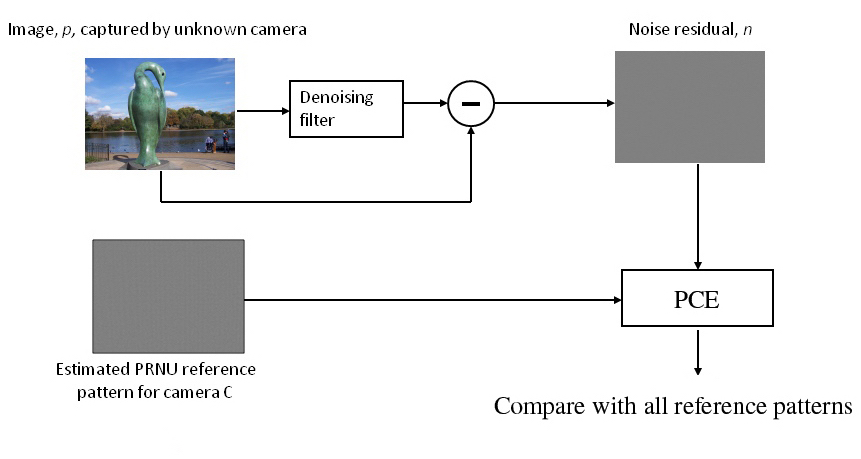
\includegraphics[width=0.8\textwidth]{../images/validation_2}
\end{center}
  \caption{Validazione delle immagini}
\label{fig:validation}
\end{figure}
\end{tframe}